\chapter{Threat Model}

We define our threat model based on the STRIDE model.
\begin{itemize}
    \item [S]poofing (Authenticity)
    \item [T]ampering (Integrity)
    \item [R]epudiation (Non-Repudiation)
    \item [I]nformation disclosure (Confidentiality)
    \item [D]enial of Service ( Availability)
    \item [E]levation of privilege (Authorization)
\end{itemize}

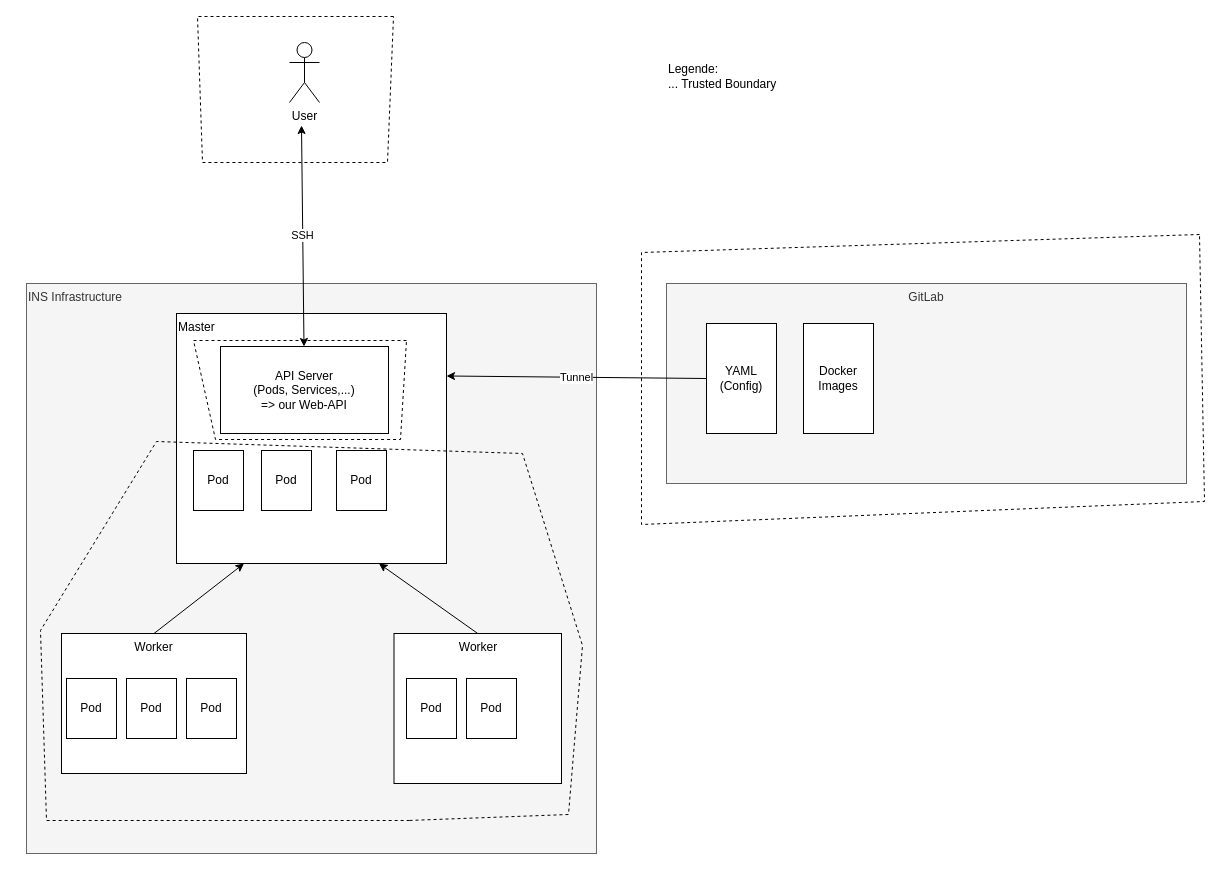
\includegraphics[height=12cm]{resources/architecture_threat_model.png}

\begin{tabular}{lllll}
    \textbf{Component} & \textbf{Category} & \textbf{Threats} & \textbf{Risk} & \textbf{Mitigation} \\
    \hline
    User                & D, E & Worm & Low & \\
                        & I & Keylogger & Low & \\
                        & & Residual risk & Low & \\
    \hline
    Interface User/Master   & I, T & Man-in-the-middle & Medium & \\
                            & I, T & SQL Injection & Medium & Input validation \\
                            & & & & Patch Services \\
    \hline
    API server          & D & Denial of Service & Medium & CPU limitation \\
                        & & & & Alerts \\
                        & & Service vulnerability (later) & & \\
    \hline
    K8 Cluster             & & & & \\
    \hline
    Interface GitLab/Master & & & & \\
    \hline
    GitLab              & & & & \\
    \hline
\end{tabular}